\chapter{Visualizations}
\label{sec:visualizations}
\INITIAL{T}{his section aims} to provide an examination of the methods used to visualize each of the most common types of data in this work. Rather than comprehensively examining all available visualizations, focus will be placed on those data types and structures which are expected to be regularly encountered. These are the data types which are not only most regularly encountered in general, but are particularly applicable to the types of computation scenarios well-suited to analyses in a map-reduce context. 
 
%%%%%%%%%%%%%%%%%%%%%%%%%%%%%%%%%%%%%%%%%%%%%%%%%%%%%%%%%%%%%%%%%%%%%%%%%%%%
%%%%%%%%%%%%%%%%%%%%%%%%%%%%%%%%%%%%%%%%%%%%%%%%%%%%%%%%%%%%%%%%%%%%%%%%%%%%

\section{Numerical Data}
\label{sec:numerical_data}
\INITIAL{N}{umerical data is ubiquitous} when it comes to analysis. Almost all tasks which involve any type of computation will have some sort of summary  or statistics to display as a result. This ubiquity has led to a myriad of visualizations being developed for similar tasks, some of which have more merit than others. The key point to consider when visualizing numerical data is to determine the purpose of the visualization. 

\paragraph{Category Comparison}
Comparing data across several categories is a task which applies to many different forms of analysis. This is best accomplished through the use of a bar chart. Bar charts display discrete groupings of typically qualitative data such as months, product categories, or ages. Rectangular bars are rendered on the horizontal axis, with the bars' heights reflecting the value assigned to their respective categories. The ordering of the bars is often arbitrary, but in cases where the bars are ordered from highest to lowest incidence the resulting chart is known as a Pareto chart. This can help to reveal trends which exist on top of being used for comparison between two individual categories. In cases where the category values are non-discrete, they can be grouped into discrete bins based on semantically sensible ranges. In this case, the resulting chart is referred to as a histogram.  

\paragraph{Pie Chart}
Another option for comparing categories is the pie chart. A pie chart is a circle which is divided into wedges representing each category, where the arc length of a wedge reflects the category's assigned value. While these charts are visually appealing, and provide an obvious visual metaphor for parts of a whole, they are generally inferior to a simple bar chart. There are several scenarios in which a pie chart becomes very difficult to read accurately. Primarily, when there are many categories, or when the categories presented are of a very similar size. In such cases, it becomes very difficult to make judgments based on the angles of the various wedges \cite{Robbins2005}. An example of this is shown in Figure \ref{fig:winepie}, in which comparing the blue wedges accurately is quite difficult visually. While it is clear that they are all roughly similar, it is particularly difficult to be certain whether Pinot Grigio and Prosecco have equal quantities, or if one is greater. This could be corrected by adding numerical labels, but the necessity for written numbers implies that a chart may not be better suited to the task than a well formatted simple table. 

%%%%%%%%%%%%%%%%%%
\begin{figure}
	\centering
	\label{fig:winepie}
	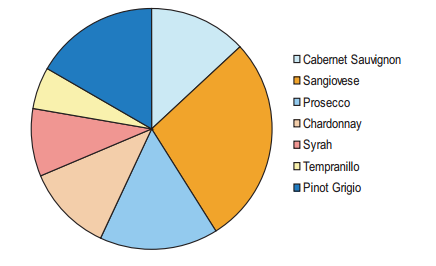
\includegraphics[scale=0.7]{pie_wine.png}
	\caption{A pie chart showing proportions of wine varieties \cite{Few2007}}
\end{figure}
%%%%%%%%%%%%%%%%%%

%%%%%%%%%%%%%%%%%%
\begin{figure}
	\centering
	\label{fig:winebar}
	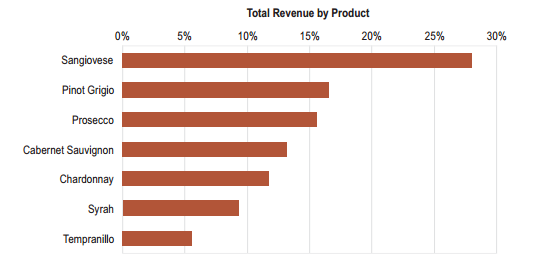
\includegraphics[scale=0.7]{bar_wine.png}
	\caption{A bar chart showing proportions of wine varieties \cite{Few2007}}
\end{figure}
%%%%%%%%%%%%%%%%%%

\paragraph{Pie Replacement}
For use in visualizing in-situ data processing in particular, we of course cannot reliably predict the proportion or in some cases number of categories in the data set. As such, it is better to assume the worst case and use a visualization which is more consistantly appropriate. Applying a percentage scale to the y-axis of a bar chart will adequately replace the visual part of whole metaphor provided by the pie chart. Aside from this, their tasks are never strongly divergent, so no other modification is necessary. Figure \ref{fig:winebar} visualizes the same data as seen in Figure \ref{fig:winepie}, using a bar chart rather than a pie. In the bar chart, the percentages are very clear and the comparison is much less ambiguous.

\paragraph{Correlation}
One of the visual analysis tasks which is best suited to human analysis is the assessment of correlation between variables. In a scenario where a data set exists with two variables, we can place each variable along an axis and mark each record as a coordinate point. Such a chart is known as a scatter plot, and suggests correlation (or lack thereof) based on the pattern of points drawn on the plot. In cases where the drawn points slope from the bottom left to the top right of the chart area, we can infer that there is a positive correlation between the two variables. Likewise, a slope from top left to bottom right implies a negative correlation. A line of best fit can be drawn on top of the scatter plot in cases where the slope is not immediately clear, or simply for clarification. 

\paragraph{Non-linear Relationships}
While seeing these positive and negative correlations is useful, it is possible to calculate them using simple methods. An even more powerful application of scatter plots is in identifying non-linear relationships between variables. For example, clusters of points are much more easily detected visually in a scatter plot than they would be through the application of statistical methods in the context of an exploratory analysis.

\paragraph{Trends} 
When examining linear trends in cases where there is a strict ordering of values on one axis, it makes sense to use a line chart. In particular, this is helpful for determining whether there is an increase or decrease in the slope of the line between individual points and through this if there is some causal relationship. Often, in cases where the trend over all data points is more important than any individual measure, sparklines can be applied. Sparklines consist exclusively of the line portion of the chart, and do not normally include axes and labeling. This is generally a design choice, and can be useful in the design of dashboards and other data-rich displays. Because of the ad-hoc nature of the analyses with which we are concerned, normal line charts will be assumed to have subsuming applicability.  

\paragraph{Summary Statistics}
There are some cases where a visualization more complex than a simple table is unnecessary and perhaps even ill-suited. When there is only a single value resulting from some aggregation, or there is nothing useful to compare resulting values to, for example. In addition, it may be the case that an analysis is complex enough that a visualization serves to further complicate understanding of the data rather than enhancing understanding. In such scenarios, it often makes sense to simply display the values on their own in comparison with other useful visualizations.

%%%%%%%%%%%%%%%%%%%%%%%%%%%%%%%%%%%%%%%%%%%%%%%%%%%%%%%%%%%%%%%%%%%%%%%%%%%%
%%%%%%%%%%%%%%%%%%%%%%%%%%%%%%%%%%%%%%%%%%%%%%%%%%%%%%%%%%%%%%%%%%%%%%%%%%%%

\section{Text Data}
\label{sec:text_data}
\INITIAL{O}{often text data is paired} with some form of numerical summary, and in many cases there is no need for a specific type of visualization for this scenario. This could be true for a data set with products and sales numbers for example, where the product names could easily be switched with an integer key and no analysis value would be lost. However, when there is semantic value which can be extracted from the text we can apply more specific techniques. Particularly, this is true if if we can present the text data itself in such a way that a viewer can assess the basic features of the data more quickly by reading the text than by using a numerical approach.

\paragraph{Word Clouds}
The most commonly encountered form of text visualization is a word cloud. Word clouds are a specific form of weighted list which were largely propagated through early blogs and websites as a common feature for exploring tags on posts. There are some examples of these visualizations appearing earlier in printed form \cite{Deleuze1987}, but these are generally not for practical analysis purposes. Word clouds can be used to either summarize the frequency with which items occur, or as a categorization method. In a frequency analysis, words within the cloud have their sizes or colours scaled to reflect their associated frequency. Categorization is applied mainly for navigational purposes, with word sizes scaling to the number of subcategories they encompass. Word clouds are often considered sub-optimal for many use cases because they remove context from the analysis and leave too much extraneous information. They still however prove quite practical for identifying flaws or unexpected features of data sets, if not for analysis. 

%%%%%%%%%%%%%%%%%%
\begin{figure}
	\centering
	\label{fig:wordcloud}
	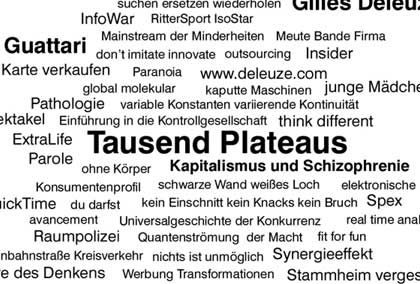
\includegraphics[scale=0.7]{tausend_plateaus_tagcloud.jpg}
	\caption{A word cloud as presented in "Tausend Plateaus: Kapitalismus und Schizophrenie" \cite{Deleuze1987}}
\end{figure}
%%%%%%%%%%%%%%%%%%

\paragraph{Word Trees}
\cite{Wattenburg2008}

\paragraph{Phrase Nets}
Phrase nets \cite{VanHam2009} represent data to some extent in the same fashion as a word cloud, with the size and colour of a word representing it's frequency in the text overall. The added benefit of a phrase net is that it also shows the relationship between words, providing greater context in later stage analyses. Rather than words floating on their own, they are connected by arrows in a directed graph. The arrows are formed based on a predefined relationship between the two and weighted in the same fashion as the words themselves, based on the frequency with which the relationship occurs. Figure \ref{fig:phrasenet} shows a phrase net built using the old testament, which connects two words X and Y based on occurences of the phrase "X of Y" in the text.

%%%%%%%%%%%%%%%%%%
\begin{figure}
	\centering
	\label{fig:phrasenet}
	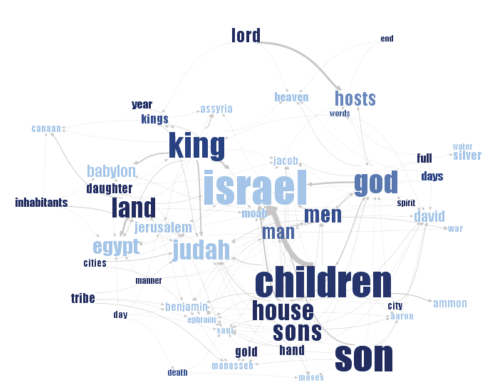
\includegraphics[scale=0.7]{phrase_net.png}
	\caption{A phrase net visualizeing "X of Y" in the old testament \cite{VanHam1987}}
\end{figure}
%%%%%%%%%%%%%%%%%%



%%%%%%%%%%%%%%%%%%%%%%%%%%%%%%%%%%%%%%%%%%%%%%%%%%%%%%%%%%%%%%%%%%%%%%%%%%%%
%%%%%%%%%%%%%%%%%%%%%%%%%%%%%%%%%%%%%%%%%%%%%%%%%%%%%%%%%%%%%%%%%%%%%%%%%%%%

\section{Graph Data}
\label{sec:graph_data}
\INITIAL{G}{raph and network} datasets are frequently topics of interest for analysts. Particularly, the subset of graph theory known as network theory provides many methods through which analysts can discover useful features of graphs. Network theory assumes that a graph is a representation of asymmetric relationships between discrete objects (as opposed to more abstract definitions as applied in graph theory generally) and has many practical real-world applications. Any area in which real networks between objects occur, such as links in computer networks, social networks, narrative connections in writing,  or even molecular networks in biology, can provide a myriad of use cases for analyses that fall under network theory. 

\paragraph{Graphs in DAG Systems}

\paragraph{KONECT}
The KONECT project \cite{Kunegis2013} at the University of Koblenz-Landau has collected a large set of network datasets and provided tools for their analysis. Their collection demonstrates that a very large number of heterogeneous data sets can be modeled as networks, and further that a generic set of analyses can be applied to these data sets if they are represented in a unified way. Though there is a taxonomy of networks based on their respective features (directed/undirected, weighted/unweighted, etc.) the vast majority of analyses are similar if not identical, and differences typically only affect the way in which analysis is performed rather than the analysis result format. Likewise, each of these analyses can be visualized in a straightforward manner.

\paragraph{Distributions}
As networks are at their core build of distinct parts, many of the relevant analyses focus on the distribution of features among the nodes or edges therein. Generally, these analyses consist of generating distributions of features across nodes or edges, and thus each can be visualized similarly. Within weighted graphs, the distribution of weights across edges in the graph provides a good representation of any skew or trends in the weighting. An example of this can be seen in Figure \ref{fig:edgeweight}. In cases where the graph is being generated during the execution of some task rather than being provided as input, such distributions can be visualized as a temporal distribution, representing a rate of change in the overall number of edges or nodes at specific points in time, such as can be seen in Figure \ref{fig:temporaldist}. Of course, these distribution analyses can be focused on other objects within the network, for example degree distributions rather than edge weight distributions. Each type of distribution will reveal some insight into either the nodes or edges of the graph. 

\paragraph{Cumulative Degree Distribution}
While distributions focus on simple aspects of a network's structure, more complex details can be extracted from the same basic data. For example, a cumulative degree distribution can be extracted to identify the probability that a randomly selected node will have a degree larger than some integer \emph{n}, as a function of \emph{n}. Such a distribution can be seen in Figure \ref{fig:cumdist}. This figure demonstrates that even as we move to more complex forms of analysis, the structure of the output data is still well suited to our basic forms of visualization. 

%%%%%%%%%%%%%%%%%%
\begin{figure}
	\centering
	\label{fig:edgeweight}
	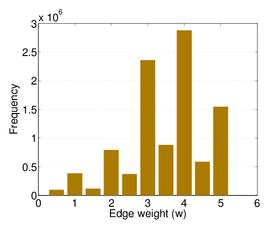
\includegraphics[scale=1.0]{edgeweight_example.png}
	\caption{A visualization of edge weight distribution \cite{KONECT2015}}
\end{figure}
%%%%%%%%%%%%%%%%%%

%%%%%%%%%%%%%%%%%%
\begin{figure}
	\centering
	\label{fig:temporaldist}
	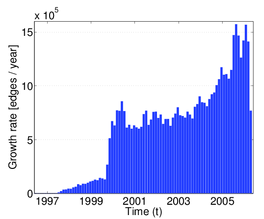
\includegraphics[scale=1.0]{temporaldist_example.png}
	\caption{A temporal visualization of edge growth \cite{KONECT2015}}
\end{figure}
%%%%%%%%%%%%%%%%%%

%%%%%%%%%%%%%%%%%%
\begin{figure}
	\centering
	\label{fig:cumdist}
	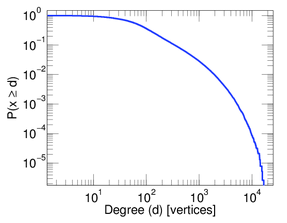
\includegraphics[scale=1.0]{cumdist_example.png}
	\caption{A visualization of cumulative distribution \cite{KONECT2015}}
\end{figure}
%%%%%%%%%%%%%%%%%%

\paragraph{Layout}
As graphs are of course a form of structural data, visualizing the structure itself is intuitive. With very small graphs this is easy to do, but as graphs grow many problems present themselves. The most obvious issue is the size itself; a graph featuring ten million nodes will be impossible to visualize in a legible way unless it has very particular features which are accounted for beforehand and visualized accordingly. In the case of even relatively small graphs, it is usually necessary to have some kind of structural information about the graph so that node placement can be handled in a sensible way during visualization. Node placement has to consider not only visibility for users, but also semantic issues such as neighbor proximity and edge overlap. Some generic methods for such problems exist, such as force-directed flow algorithms \cite{Didimo2011}, but it is difficult to predict their efficacy in ad-hoc scenarios where the graph's structure is unknown.
 

%%%%%%%%%%%%%%%%%%%%%%%%%%%%%%%%%%%%%%%%%%%%%%%%%%%%%%%%%%%%%%%%%%%%%%%%%%%%
%%%%%%%%%%%%%%%%%%%%%%%%%%%%%%%%%%%%%%%%%%%%%%%%%%%%%%%%%%%%%%%%%%%%%%%%%%%%

\section{Summary}
\label{sec:vis_summary}
\INITIAL{L}{ooking at the scenarios} presented in the previous section, it becomes clear that the vast majority of visualization scenarios which would be encountered during exploratory or in-situ processing can be handled using very basic tools. Specifically, these include bar charts, line charts, scatterplots, and simple mutations of each. 